%%%%%%%%%%%%%%%%%%%%%%% file template.tex %%%%%%%%%%%%%%%%%%%%%%%%%
%
% This is a general template file for the LaTeX package SVJour3
% for Springer journals.          Springer Heidelberg 2010/09/16
%
% Copy it to a new file with a new name and use it as the basis
% for your article. Delete % signs as needed.
%
% This template includes a few options for different layouts and
% content for various journals. Please consult a previous issue of
% your journal as needed.
%
%%%%%%%%%%%%%%%%%%%%%%%%%%%%%%%%%%%%%%%%%%%%%%%%%%%%%%%%%%%%%%%%%%%
%
% First comes an example EPS file -- just ignore it and
% proceed on the \documentclass line
% your LaTeX will extract the file if required
\begin{filecontents*}{example.eps}
%!PS-Adobe-3.0 EPSF-3.0
%%BoundingBox: 19 19 221 221
%%CreationDate: Mon Sep 29 1997
%%Creator: programmed by hand (JK)
%%EndComments
gsave
newpath
  20 20 moveto
  20 220 lineto 
  220 220 lineto
  220 20 lineto
closepath
2 setlinewidth
gsave
  .4 setgray fill
grestore
stroke
grestore
\end{filecontents*}
%
\RequirePackage{fix-cm}
%
%\documentclass{svjour3}                     % onecolumn (standard format)
%\documentclass[smallcondensed]{svjour3}     % onecolumn (ditto)
\documentclass[smallextended]{svjour3}       % onecolumn (second format)
%\documentclass[twocolumn]{svjour3}          % twocolumn
%
\smartqed  % flush right qed marks, e.g. at end of proof
%
\usepackage{graphicx}
\graphicspath{{figures/}}
%
% \usepackage{mathptmx}      % use Times fonts if available on your TeX system
%
% insert here the call for the packages your document requires
%\usepackage{latexsym}
\usepackage{subfigure} % subfiguras
\usepackage{svg}
\usepackage{caption}
%\usepackage{subcaption}
\usepackage{geometry}
\usepackage{amsmath,amssymb}
\usepackage{listings}
\usepackage{xcolor}
\usepackage{mdframed} %nice frames
\usepackage[shortlabels]{enumitem} %cambiar enumeración de items por letras o numeeros
\usepackage{setspace}

%
% please place your own definitions here and don't use \def but
%Definiciones
%\newtheorem{theorem}{Theorem}%[section]
%\newtheorem{corollary}{Corollary}%[theorem]
%\newtheorem{lemma}{Lemma}%[theorem]
%\newtheorem{definition}{Definition}%[section]
%
% Insert the name of "your journal" with
\journalname{Engineering with Computers}

%	\doublespacing

\begin{document}

\title{Polygon meshing algorithm based on terminal-edge regions}%\thanks{Grants or other notes
%about the article that should go on the front page should be
%placed here. General acknowledgments should be placed at the end of the article.}

%\subtitle{Se puede llamar algoritmo del cuyi \\ o algo relacionado con cuyis?}

%\titlerunning{Short form of title}        % if too long for running head

\author{Sergio Salinas       \and
        Nancy Hitschfeld-Kahler \and Hang Si  \and Alejandro Ortiz-Bernardin %etc.
}

%\authorrunning{Short form of author list} % if too long for running head

\institute{Sergio Salinas \at
        University of Chile\\
              \email{ssalinas@dcc.uchile.cl}           %  \\
%             \emph{Present address:} of F. Author  %  if needed
           \and
           Nancy Hitschfeld \at
              University of Chile\\
              \email{nancy@dcc.uchile.cl}
            \and
             Alejandro Ortiz-Bernardin \at
              University of Chile\\
              \email{aortizb@uchile.cl}
            \and    
             Hang Si \at
              Weierstrass Institute for Applied Analysis and Stochastics (WIAS)\\
              \email{si@wias-berlin.de}      
}

\date{Received: date / Accepted: date}
% The correct dates will be entered by the editor


\maketitle

\begin{abstract}
\textcolor{blue}{This paper is a study of a new kind of polygon mesh obtained from a Delaunay triangulation using the concept of terminal-edge region. An algorithm to generate those meshes is proposed. The algorithm is divided into three phases and takes as input a Delaunay triangulation. The first phase is to label each edge and triangle of the input triangulation; the second phase is to build polygons (simple or not) from terminal-edges region using the label system; and the third phase is to transform each non simple polygons into simple ones. The final mesh contains polygons with convex and non convex shape. Due to the similarities with the Voronoi diagram, this paper also explores empirical properties and comparisons between our proposed meshes and Clipped Voronoi meshes are studied. Finally, we validate these new terminal-edge based polygon meshes by solving a Laplace equation on an L-shaped domain using the Virtual Element Method (VEM) and demonstrate the optimal convergence rate of the numerical solution.}

%To generate each polygon, the algorithm uses classification of each edge of a Delaunay triangulation; second it uses the classification to generate terminal-edges and builds polygons (simple or not) with the


%\textcolor{blue}{This paper is a study on a new kind of polygon mesh obtained from a Delaunay triangulation using the concept of Terminal-edge region}. To generate each polygon, the algorithm starts by generating a Delaunay triangulation of a point set; second it builds polygons (simple or not) from terminal-edge regions, and third it transforms each non simple polygon into simple ones. The final mesh contains polygons with convex and not convex shape. Due to the similarities with Voronoi Diagram, this paper also explores comparisons and empirical properties between our mesh and \textcolor{blue}{Clipped Voronoi mesh. Finally, we validate our mesh testing it with the Virtual Element Method (VEM) given the exact solution in~\cite{MITCHELL2013350}.}   

%  We analyse which kind of non simple polygons appear and show the algorithm to divide them into simple ones.  Some empirical properties of the resulting meshes are shown.
\keywords{First keyword \and Second keyword \and More}
% \PACS{PACS code1 \and PACS code2 \and more}
% \subclass{MSC code1 \and MSC code2 \and more}
\end{abstract}

\section{Introduction}

\textbf{Meshes based on triangles and quadrilaterals are common in simulations using the Finite Element Method (FEM). The problem is that polygons(elements) in FEM need to obey specific quality criteria, to avoid angles that are too large or small, or with sides of graded  length (aspect ratio criteria), etc. To fulfill these criteria, sometimes the insertion of a large number of points and elements is required in order to properly model a domain, increasing the time needed to make the simulation. New methods as Virtual Element Method (VEM)~\cite{Basisprinciples,Brezzi2015} can use any polygon as basic cell. So, (i) the domain geometry can be fitted using  less elements than if only triangles and quadrilaterals are used, (ii) the required point density distribution is just that required by the simulation problem, and (iii) it should not be necessary to further improve the quality of the elements. We are currently researching how far the VEM can allow the simulation of more complex problems, in both 2D and 3D, in comparison to FEM~\cite{Wriggers2019}.}

%pregunta

%motivación

% contribución

%org


%---- Actualmente se usan las mallas basadas en el diagrama de voronoi, poligonos convexos. Se ha probado insertando poligonos aislados no convexos y evaluar si los resultados de la silumlacin son aun validos...Wriggers2017...

%---- las preguntas our research questions sn... podemos generar poligonos arbitrarios, automaticantes a partir de una geometria PSLG...y puntos interiores dados como input? .. ..

In this paper we propose an algorithm to generate meshes with polygons of arbitrary shape (convex and non-convex) based on the label system described in~\cite{Ojeda2018ANA}. These meshes might contain non-simple polygons, so we also propose an algorithm to repair them. We  experiment to show the properties of these polygons, compare these meshes with Clipped Voronoi meshes, and we validate our mesh to shows that it works with the VEM. \textcolor{blue}{The algorithm needs an initial triangulation as input, therefore we choose uses the Delaunay triangulation as input, as Delaunay triangulation is the triangulation with the maximal angles, then the resulting mesh has the maximal angles too.}

Our motivation is the generation of meshes that adapt to a geometric domain using  polygons of any shape, but respecting the required point density. To do this, we propose to use the concept of terminal-edge region. Our main research questions are: Can terminal-edge regions be adapted to be used as good basic cells for polygon numerical methods such as VEM? Do these kinds of meshes need less polygons to model the same problem than polygon meshes based on the Voronoi diagram? 

%
\textcolor{blue}{Thus, the main contributions of this paper are: A simple and automatic way to generate polygon meshes of arbitrary shape, without adding additional points to the initial input, and a evaluation of our meshes in tested simulations with the VEM.}


This paper is organized as follows: Section~\ref{sec:relatedwork} shows the state of art;  Section~\ref{sec:basic} introduces the basic concepts to understand the algorithm; in Section~\ref{sec:the_algorithm} there is a description of the algorithm divided in three main phases and the data structure used in its implementation in C++; Section~\ref{sec:experimental_evaluation} shows experiments of the algorithm to do a comparison with Clipped Voronoi meshes; Section~\ref{sec:simulation_results} shows a assessment of the meshes in the Virtual Element Method (VEM) and Section~\ref{sec:conclusions} explains the conclusions and ongoing work.

%Section~\ref{sec:experimental_evaluation} shows a preliminary experimental evaluation of the generated meshes  on random points, some  properties of the polygons and  a comparison  with Voronoi based meshes. Section \ref{sec:Conclusions} shows the ongoing work.

\section{Related work}
\label{sec:relatedwork}
%REVISAR Y DEJAR REFERENCIAS 2D

%\textcolor{blue}{To our knowledge, there are no algorithm to automatized the generation of 2D meshes with arbitrary shape for {\sc vem}}. 

\textcolor{blue}{To our knowledge, there are no algorithms to automatized generation of 2D meshes with arbitrary shape for {\sc vem}. There have been interesting methods of generating meshes \cite{PackingJoaquin}, where a packing-based mesh was proved functional to work with {\sc vem}.} %But interesting methods to generate meshes as been tested, in \cite{PackingJoaquin} a packing-based mesh was proved being functional to work with {\sc vem}. 

In the case of the standard finite element method, the most used 2D meshes are triangulations~\cite{chew1,Shewchuk96,Detri2} or quadrilateral meshes~\cite{Canann98,Lee20031055,Owen98advancingfront}. 2D Mixed meshes composed of triangles and quadrilaterals have also been used, but are not so common~\cite{gildaDiss} as the previous ones. Other methods use the Voronoi diagram as the polygon/polyhedron mesh, and the Voronoi cells as mesh elements are presented in~\cite{YanWLL10,EbeidaM11,SiegerAB10}.
 
The generalization of finite element methods to include polygons/polyhedra as part of the mesh elements was started in the last decade ~\cite{Sukumar2006,tabarraei2008extended,NATARAJAN2017218}.  Polygonal elements are usually generated by using a quadtree approach and from Voronoi cells. The {\sc vem} was introduced seven years  ago~\cite{Basisprinciples,Brezzi2015} and since then, several research groups have been developing computational frameworks  for using the {\sc vem}, both in 2D and 3D, in order to explore how far the {\sc vem} can be used to solve new problems. To mention some  examples, the {\sc vem} has been formulated and applied to solve linear elastic and inelastic solid mechanics problems~\cite{da2015virtual}, in fluid mechanics~\cite{caceres2015mixed}, in the optimization
of  a fluid problem through a discrete network~\cite{benedetto2014virtual}, for compressible and incompressible nonlinear elasticity~\cite{Wriggers2017}, for finite elasto-plastic deformations~\cite{Wriggers2017a} and brittle crack propagation~\cite{HUSSEIN201915}.
%% Since we are going to explore


%meshes has been testing with VEM besides Voronoi meshes, in \cite{PackingJoaquin} a packing-based mesh was tested. 
\section{Basic concepts}
\label{sec:basic}


%Given a conforming Delaunay triangulation $CDT(\Omega)$, for each triangle $t \in CDT(\Omega)$ is possible to define a longest-edge, in the case of equilateral and isosceles triangles, the equal length edges are arbitrarily ordered. 
The proposed polygon meshing algorithm is based on two concepts: Longest-edge propagation path (Lepp) introduced in~\cite{Rivara97} and terminal-edge regions defined in~\cite{Ascom209}. These concepts and some related properties are briefly reviewed in this section.

\subsection{Terminal-edge regions}

In any triangulation, triangles can be grouped under the Longest-edge propagation path concept defined as follows:



\begin{definition}{\textbf{Longest-edge propagation path }~\cite{Rivara97}:}\label{d:lepp}  
For any triangle $t_0$ in any triangulation $\Omega$, the Lepp($t_0$)
%\emph{Longest-Edge Propagation Path} of $t_0$  (Lepp($t_0$))
is the ordered list of all the triangles $t_0$, $t_1$, $t_2$, ..., $t_{l-1}$, $t_{l}$, such that $t_{i}$ is the neighbor triangle of $t_{i-1}$  by the longest-edge of $t_{i-1}$, for $i = 1,2,\dots,l$. The longest-edge shared by $t_{l-1}$ and $t_l$ is a terminal-edge and $t_{l-1}$ and  $t_l$ are terminal-triangles. If the longest-edge   \textcolor{blue}{An example of the lepp of a triangle is shown in Figure \ref{fig:leppex1}.}
\end{definition}



\begin{figure}[h]
\centering     %%% not \center
\subfigure[Lepp example]{\label{fig:leppex1}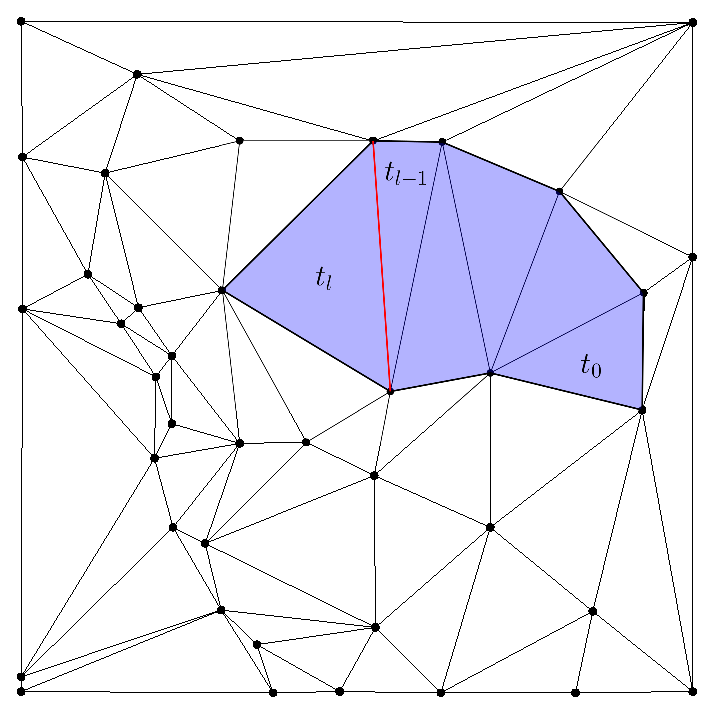
\includegraphics[width=0.3\textwidth]{leppex1.eps}} 
\subfigure[Multiple Lepp with same terminal-edge]{\label{fig:leppex2}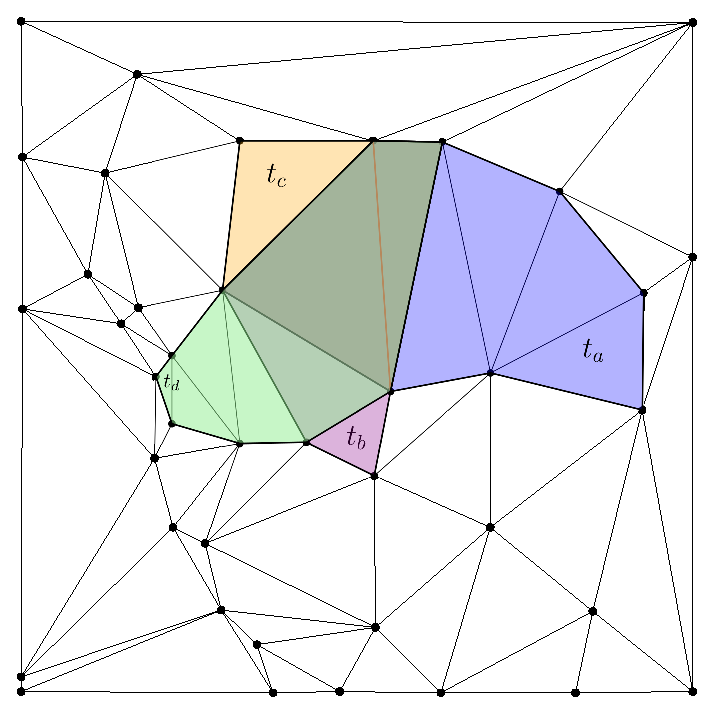
\includegraphics[width=0.3\textwidth]{leppex2.eps}}
\subfigure[Terminal-edge region]{\label{fig:leppex3}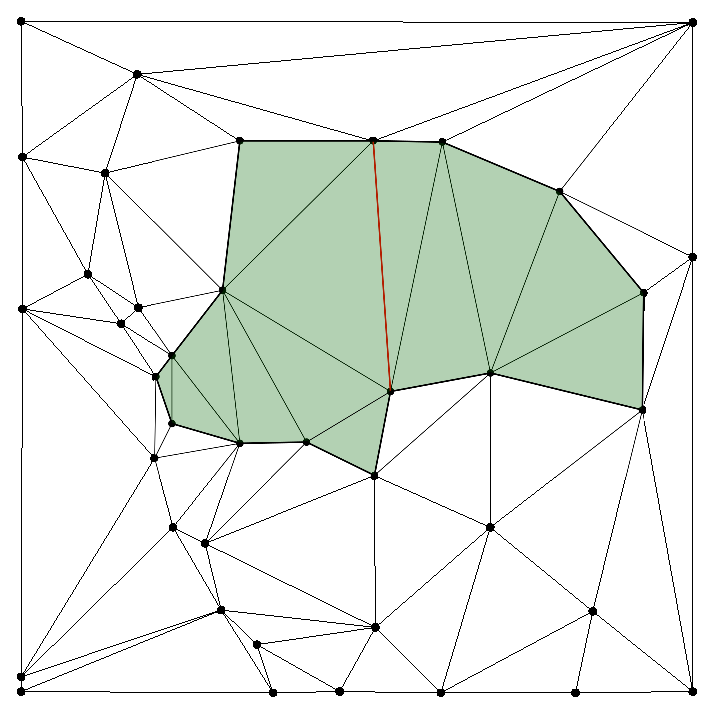
\includegraphics[width=0.3\textwidth]{leppex3.eps}}
\caption{Generation of terminal-edge regions \textbf{(a)} Longest-edge propagation of $t_0$, red line is a terminal-edge. \textbf{(b)} Four diferents lepp, Lepp($t_a$), Lepp($t_b$), Lepp($t_c$) and Lepp($t_d$), with the same terminal-edge. \textbf{(c)} Union of Lepp($t_a$),..., Lepp($t_d$) to generate a terminal-edge region.}
\label{fig:leppexample} 
\end{figure}

\noindent
Moreover, triangle edges can be classified according to their edge lengths inside the two triangles that share them. Therefore, given an edge $e$ and two triangles $t_1$, $t_2$ that share $e$, we can label  $e$ as: 

\begin{itemize}
    \item Terminal-edge~\cite{Rivara97}, if $e$ is the longest-edge of $t_1$ and $t_2$.
    \item Frontier-edge~\cite{Ascom209}, if $e$ is neither the longest-edge of $t_1$ nor $t_2$.
    \item Internal-edge, if $e$ is the longest edge of $t_1$ but not of $t_2$ or vice-versa.
\end{itemize}


In case of equilateral or Isosceles triangles, one edge is chosen arbitrary as the longest-edge. \textcolor{blue}{ Boundary edges, by simplicity, are considered as frontier-edge.}


\begin{definition}{\textbf{Terminal-edge region~\cite{Ascom209}:}}
\label{d:terminaledgeregion}
A {\em terminal-edge region} $R$ is a region formed by the union of all triangles $t_i$ such that Lepp($t_i$) has the same terminal-edge.  In case that the terminal-edge region  is delimited by a boundary-edge the region will be called {\em boundary terminal-edge region}. \textcolor{blue}{ Figure \ref{fig:leppexample} shows the generation of terminal-edge region. Figure \ref{fig:leppex2} shows four lepp with same terminal-edge, the union of those lepp generates a terminal-edge region in Figure \ref{fig:leppex3}.}
\end{definition}


\noindent
Terminal-edge regions have some properties already proven. Important properties for the understanding of the algorithm proposed below, are: 

\begin{itemize}
    \item Terminal-edge regions are surrounded by frontier-edges~\cite{Ascom209}.
    \item Terminal-edge regions cover the whole domain without overlapping~\cite{Ascom209}~\cite{Ojeda2018ANA}.
    \item Terminal-edge-regions might include frontier-edges in their interior. We have called this kind of frontier-edge a \textbf{Barrier-edge}~\cite{Ascom209}~\cite{Ojeda2018ANA}.
  
\end{itemize}
\noindent

%{\bf SERGIO: REVISAR EN EL PAPER SI HAY OTRAS PROPIEDADES UTILES}

%{\bf mencionar que pasa con triangulos equilateros}

\noindent
Figure \ref{fig:general_example} shows those properties. Figure~\ref{fig:initialpoinset} shows a set of points; Figure~\ref{fig:labelsystem} shows the Delaunay triangulation of this point set when terminal-edges are drawn using red dashed lines: internal-edges using black dashed lines and frontier-edges using  solid lines and Figure~\ref{fig:terminalregion} shows each terminal-edge region using a different color. We observe in Figure~\ref{fig:terminalregion} terminal-edge regions are enclosed by frontier-edges and the green region includes a barrier-edge.



\begin{figure}[h]
\centering     %%% not \center
\subfigure[Initial point set]{\label{fig:initialpoinset}\includegraphics[width=0.3\textwidth]{delaunaypoints.eps}} 
\subfigure[Delaunay triangulation]{\label{fig:labelsystem}\includegraphics[width=0.3\textwidth]{delaunaylabel.eps}}
\subfigure[Terminal-edge regions]{\label{fig:terminalregion}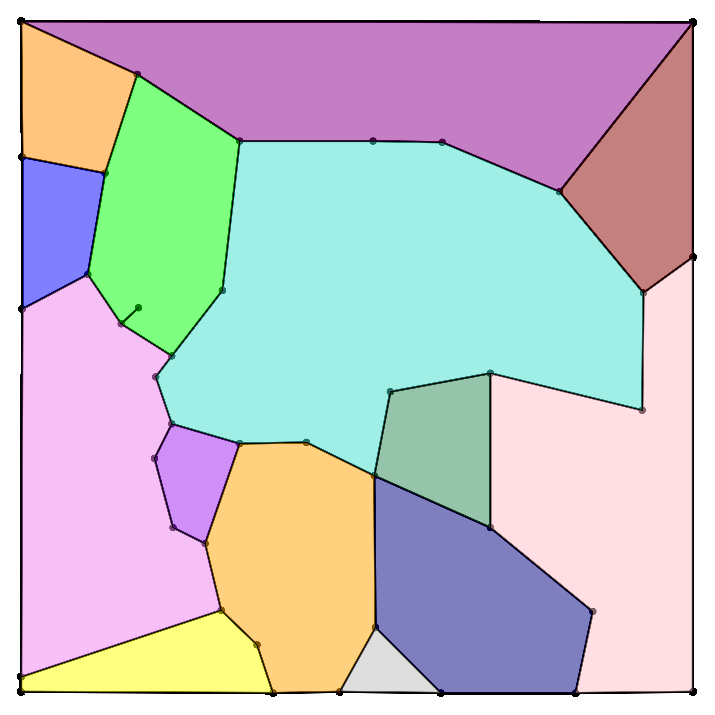
\includegraphics[width=0.3\textwidth]{delaunaylabelcolors}}
\caption{(a) Initial random point set. (b) Delaunay Triangulation: Solid lines are frontier-edges, dashed black lines are internal-edges and red dashed edges are terminal-edges. (c) Terminal-edge regions}
\label{fig:general_example} 
\end{figure}

\subsection{Terminal-edge regions as  polygons}

%\textbf{A esto le falta intro y decir porque es importante nombrarlo}

Because one of their proprieties of terminal-edge regions is that they covert a geometric domain without overlapping, means that they can be used to generate polygon meshes, representing each terminal-edge regions as polygons, simple and non-simple polygon. Non-simple polygons appear when terminal-edge regions include barrier-edges.  As observed in Figure~\ref{fig:general_example}, the domain can be tessellated into 14 polygons where only the green region is represented by a  non-simple polygon: it includes one barrier-edge. 
%\begin{figure}
%    \centering
%    \includegraphics[width=0.5\textwidth]{delaunaylabel.eps}
%    \caption{Terminal-edge regions: Solid lines are frontier-edges, dashed black lines are internal-edges and red dashed edges are terminal-edges.}
%    \label{fig:general_example}
%\end{figure}



\noindent
For simplicity, in the case  $e$ is a domain boundary edge, $e$ will be considered a frontier-edge too (see the edges belonging to the square in Figure \ref{fig:general_example}(b) and (c)). 
  
%\begin{definition}{\textbf{Barrier-edge:}}
%\label{d:barrier-edge}
%A {\em barrier-edge} is a especial kind of frontier-edge: the %triangles that share it belong to the same terminal-edge %region. The barrier-edges generate  non-simple polygon as shown %in Figure \ref{figs:kindofbarrieredges}.
%\end{definition}

In order to build a conforming polygon tessellation from the partition generated from terminal-edge regions, non-simple polygons must be divided into simple polygons. That requires the integration of barrier-edges as part of the boundary of new simple polygons.  Since this requirement is part of the meshing algorithm we are proposing in Section~\ref{sec:the_algorithm}, we need, beforehand, to introduce some definitions and prove some properties that will sustain the construction of the algorithm.


\begin{definition}{\textbf{Barrier-edge tip:}}
\label{d:barrier-edge}
A barrier-edge tip in a terminal-edge region $R$ is a barrier-edge endpoint shared by no other barrier-edge%4 nor frontier-edge. See Figure \ref{figs:kindofbarrieredges}.\\
\end{definition}

%{\bf SERGIO: Marcar los barrier edge tips en la figura y describir mejor cada caso en el texto!!!!}
 
In Figure \ref{figs:kindofbarrieredges} we can see two polygons with barrier-edges, barrier-edge tips are shown in the color green. Figure \ref{fig:1be} shows a basic case of polygon with barrier-edge tips and Figure \ref{fig:2be} a case with two barrier-edge tips, there is no limit to the maximum number of barrier-edges for a polygon. Each point of the input is an endpoint of a frontier-edge or barrier-edge. Terminal-edge regions have none isolated interior points. Barrier-edge tips belong to a barrier-edge. Lemma~\ref{l:verticeslemma} demonstrates this property.

\iffalse
\begin{figure}[h]
\centering  
\resizebox{.8\linewidth}{!}{
   %%% not \center
\subfigure[One barrier-edge and one tip] {\label{fig:1be}\includegraphics[width=0.2\textwidth, ]{simplebe.eps}}\hspace{0.5cm}
\subfigure[Four barrier-edges and two tips]{\label{fig:2be}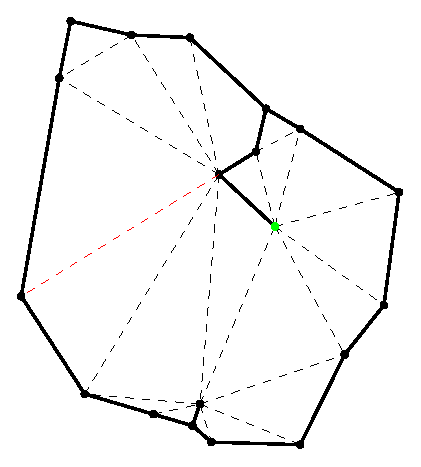
\includegraphics[width=0.22\textwidth, angle =60]{nosimplebe.eps}}\hspace{0.5cm}
\subfigure[Two barrier-edges and one tip]{\label{fig:1beequi}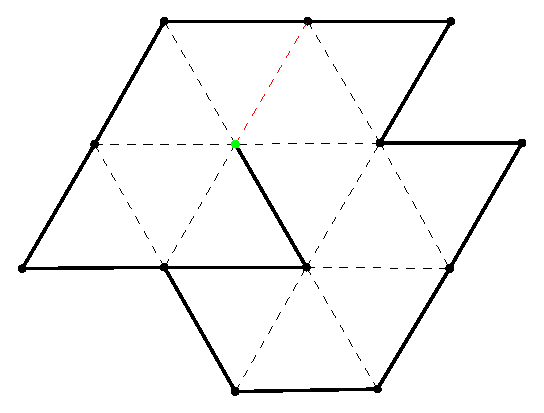
\includegraphics[width=0.28\textwidth]{equiratelbe.eps}}
}
\caption{Examples of non-simple polygons with barrier-edges. Black lines are frontier-edges, dashed black lines are internal-edges and red edges are terminal-edges. \textbf{(a)} One barrier-edge tip \textbf{(b)} Two barrier-edges tips. }
\label{figs:kindofbarrieredges} 
\end{figure}
\fi

\begin{figure}[h]
\centering  
\subfigure[One barrier-edge and one tip] {\label{fig:1be}\includegraphics[width=0.15\textwidth, ]{simplebe.eps}}\hspace{2cm}
\subfigure[Four barrier-edges and two tips tip]{\label{fig:2be}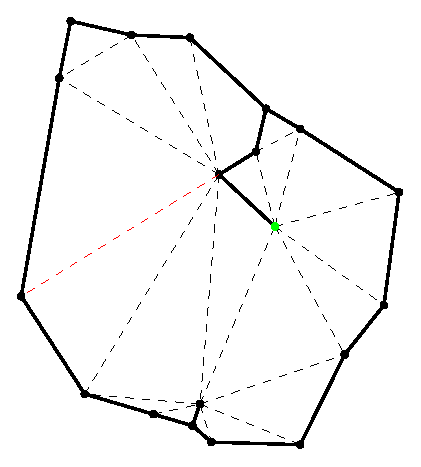
\includegraphics[width=0.15\textwidth, angle =60]{nosimplebe.eps}}\hspace{0.5cm}

\caption{Examples of non-simple polygons with barrier-edges. Black lines are frontier-edges, dashed black lines are internal-edges and red edges are terminal-edges. \textbf{(a)} One barrier-edge tip \textbf{(b)} Two barrier-edges tips. }
\label{figs:kindofbarrieredges} 
\end{figure}




%\begin{wrapfigure}{l}{0.4\textwidth}

%\centering
%\includegraphics[width=0.9\linewidth]{demostracionlemma2.1} 
%\caption{Green vertex is not part of a frontier-edge.}
%\label{fig:lemmaquitadomingos}
%\end{wrapfigure}

\begin{lemma}\label{l:verticeslemma}
Let us  $\Omega$ be a triangulation with a set of vertices $V$ \textcolor{blue}{in general position}. Then, each vertex $v$ is an end-point of at least one  of  the  frontier-edge or barrier-edges and  there is no isolated interior points \textcolor{blue}{(vertices incident only to internal-edges)}.
\end{lemma}

\textbf{Proof:} Let $v$ be  a vertex  associated to the terminal-edge region $R$ generated by the terminal-edge $e$ and  $T$ the set of the triangles that share $v$. By contradiction, lets assume that $v$ is an interior point of $R$ as shown  in Figure \ref{fig:lemmaquitadomingos}. Since the triangles in $T$ are part of $R$, they must share their longest-edge around $v$. 
%with as predecessor  one of the triangles that contains $e$. All edges incidents to $v$ are internal-edges. 
Given that $T$ is finite, there should exist a triangle $t_0$ (see Figure \ref{fig:lemmaquitadomingos}) that shares their longest-edge with two triangles of $R$ in order to maintain $v$ interior point in $R$. This is not possible because a triangle has just one edge labeled as its  longest-edge. This contradicts our assumption, so $v$ has to be an endpoint of  at least one frontier- or barrier-edge of $R$. \textcolor{blue}{ As $\Omega$ is partitioned into terminal-edge regions $R_i$ without overlap~\cite{Ojeda2018ANA}, then there can not exists isolated points in $\Omega$.} \qed

\begin{figure}[h]
\centering
\includegraphics[width=0.25\linewidth]{demostracionlemma2.1} 
\caption{The  vertex in green is an interior point.}
\label{fig:lemmaquitadomingos}    
\end{figure}


It is worth mentioning that Lemma \ref{l:verticeslemma} is important, since it means that the initial points used to represent the geometric domain and the ones inside the domain to fulfill point density requirements, are maintained after the polygon mesh is generated. Moreover, it allows for the use of interior-edges that contain barrier-edge tips as endpoints to split a non-simple polygon into simple polygons.
\newpage
\textcolor{blue}{There is a degenerate case that does not respect Lemma \ref{l:verticeslemma}, when points are not in general position. Given a vertex $v$ of a triangulation $\Omega$ and $T$ the set of triangles incident to $v$. If all triangles in $T$ are equilateral, it may happen that the algorithm chooses all the left edges or all right edges as longest-edge in triangles $T$, generating a circular lepp without terminal-edge and the final mesh would have a hole. This rare case can be solve changing the order in that arbitrary longest-edge is selected in the algorithm.}


\section{The algorithm}
\label{sec:the_algorithm}

%The algorithm receives as input a Constrained Delaunay triangulation $CTD(\Omega)$ and generates as output a polygon mesh.  Algorithm consists in three main steps:

In this section, we describe  the main steps of the proposed algorithm, its computational cost  and the data structure used for its implementation.
The algorithm receives an initial triangulation as input, that can be generated by any known triangulator. The triangulation can be Delaunay or not, but we are using Delaunay triangulations because, \textcolor{blue}{ as Delaunay triangulation is the triangulation with the maximal angles, then the resulting mesh has the maximal angles too. Also several correct and robust triangulators} such as Detri2~\cite{Detri2} and Triangle~\cite{Shewchuktriangle} are available for free.  We use Detri2 \cite{Detri2} to generate the constrained Delaunay triangulations used as initial mesh. The whole process applied to the initial triangulation is divided in three phases:


\begin{enumerate}[label=\roman*)]
    \item Label phase: Each edge is labeled as  longest-, terminal or frontier edges. Also the algorithm labels seed triangles used in the next phase.
    \item Traversal phase: Generation of polygons from seed triangles. \textcolor{blue}{In this phase frontier-edges of a terminal-edge region are store as part of the new polygon. Non-simple polygons generate in this phase are sent to the partition phase.}
    \item Partition phase: Polygon with barrier-edges are partitioned into simple polygons.
\end{enumerate}


\subsection{Data structures}
\label{sec:datastructrue}
%\textbf{Mover la estructura de datos dentro del algoritmo, ponerlo depsués del análisis de complejidad}
In this subsection we show the data structures used in a implementation in C++ and its highlights to  contribute to a better understanding of the algorithm.  %Also we show the result of the experiments and examples of the kind of meshes that the algorithm can generate.

%\subsection{Data structures}
%\label{subsec:datastructrue}


To represent the Delaunay triangulation, three one-dimensional arrays are used to represent  vertices, triangles and adjacent triangles respectively.

Vertices are saved in pairs $(x,y)$, where each two elements of the array are the coordinates $x$ and $y$ of a vertex. Triangle array is set of indices to the Vertex array. Each 3 values is a triangle in the array. Since the algorithm needs to know the neighbor of each triangle, an array is used to save the indices to adjacent triangles: each 3 values in this array $3i + 0$, $3i + 1$, $3i + 2$ are the indices to the triangle of adjacent triangle $i$. 

To facilitate the implementation of the algorithm, indices in the triangle array are ordered based on adjacent triangles, in such a manner that is easy find out, in a side triangle, whose points are shared with the adjacent triangle.  The order is shown in the Figure \ref{figs:data_and_triangle} and it is similar to that used by Detri2 \cite{Detri2}. The first two point indices $3i+0$, $3i+1$ in Triangle array are shared with its adjacent triangle in the position $3i+2$ of Adjacent array, points $3i+1$, $3i+2$ in Triangle array with element $3i+2$ in Adjacent array and elements $3i+1$, $3i+2$ in Triangle array with element $3i+1$ in Adjacent array. This is also an implicit way to identify each edge in a triangle, being the red edge of Figure \ref{figs:data_and_triangle} the edge 0, blue the edge 1 and green the edge 2.  \textcolor{blue}{To label edges as frontier-edge the algorithm mark the adjacency as $-1$. For example, in Figure \ref{figs:data_and_triangle}, to label red edge as frontier edge, $ADj_{3i+0}$ must change its value by $-1$. }

\begin{figure}
\centering     %%% not \center
\subfigure[Data structure]{\label{fig:datastruc}\includegraphics[width=0.3\textwidth]{data_struc_withpoints.png}}\hspace{2cm}
\subfigure[Triangle]{\label{fig:datastructriangle}\includegraphics[width=0.3\textwidth]{triangulo.png}}
\caption{Data structure:  \textbf{(a)} Relation between the order in Triangle array and the elements in Adjacent array. \textbf{(b)} The parts of a triangle represented in Triangle array and Adjacent array. In the case of Adjacent array, the elements store both the edges and  the adjacent triangle to that edge.}
\label{figs:data_and_triangle} 
\end{figure}




In the label phase, a seed lists is defined, it is a integer list that contains the indices of the triangles labeled as seed at the end of first phase. In the case of the reparation phase, one open hash table $H$, without repeat elements, is used instead of a seed list to store the indices of triangles that will generate new polygons.

\begin{figure}
\centering     %%% not \center
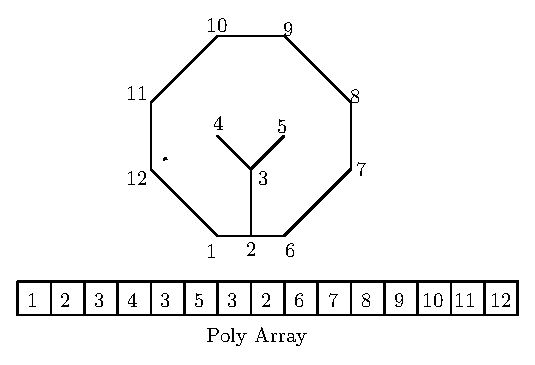
\includegraphics[width=0.4\textwidth]{polyarray.eps} 
%\subfigure[Data structure]{\label{fig:b_data_poly}\includegraphics[width=0.31\textwidth]{datastructure_split2}}
%\subfigure[Data structure]{\label{fig:c_data_poly}\includesvg[width=0.3\textwidth]{datastructure_split3.svg}}
\caption{Representation of polygon as set of vertices. Sequences $3 - 4 - 3$ and $3 - 5 - 3$ indicate the existence of barrier-edge tips.}%\textbf{(b)} Simulation of addition of an edge to calculate the optimal distance.}
\label{fig:a_data_poly} 
\end{figure}


%a integer list of length equal to the number of terminal-edges,  (they are store in label phase) and  % To simulate splits of polygon, the algorithm search the initial point and the endpoint of the edge to add in the array of the polygon and generate two polygons to calculate the optimal area as is show in Figure \ref{fig:b_data_poly}. 

In the travel phase, polygons are temporally stored in an array with the vertices that conform it as is shown in Figure \ref{fig:a_data_poly}, \textcolor{blue}{ store one edge in a polygon means adding their to endpoints in counter-clock wise to the temporal array that represents that polygon}. After generate each non-simple polygons, they are stored in a mesh. The mesh consists in just one array, where each polygon stores first its length (number of vertices) and after the index of their vertices as is shown in Figure \ref{fig:meshdatastruct}. To improve the compute of $deg(b_i)$ we added an array that pair each vertex to one triangle adjacent to that vertex to the algorithm.

\textcolor{blue}{All mentioned arrays, list and tables uses $O(n)$ of memory space, where $n$ is the number of points.}

%To the reparation phase a recursive function had been chosen to split polygons (split a polygon in two, and those two split them again until removing all barrier-edge tips), but to optimise the use of memory a open hash table $H$ was use. This table is an array of arbitrary length with pointers to linked list where save the seed triangles uses to generate the new polygons where each element is added to the begin of the linked list and each search operation has a delete operation inside to remove already use triangles.

\begin{figure}[]
    \centering
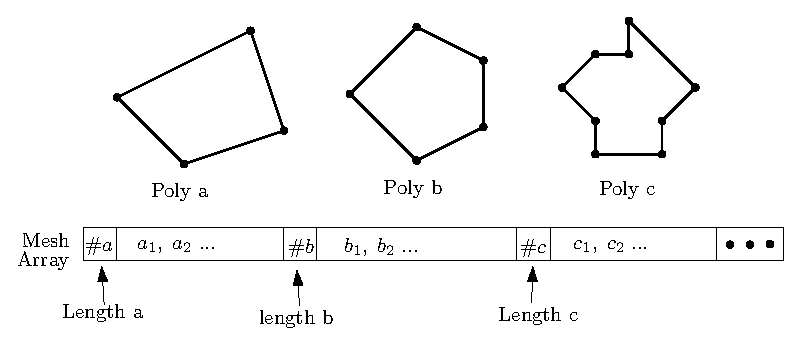
\includegraphics[width=0.7\textwidth]{meshdatastruct.eps}
    \caption{Mesh array with three polygons.} 
    \label{fig:meshdatastruct}
\end{figure}

\subsection{Label Phase}
\label{subsec:Labelpohase}

The Label phase refers to labeling each edge of a triangle as a frontier edge or not and looking for triangles to use in the next phase to generate polygons. Those triangles are called seed triangles.

The algorithm first cycles over each triangle of the initial triangulation to compute which edge is the longest-edge; in the case of equilateral and isosceles triangles the algorithm chooses randomly any edge as the longest-edge. This step avoids having a triangle belong to two terminal-edge regions at the same time. 

Afterward, the algorithm does a second iteration over the edges. In the case when an edge $e$ is not the longest-edge of any of the two triangles that share it, $e$ is labeled as a frontier-edge. In this iteration the algorithm also labels seed triangles. In the case when $e$ is a terminal-edge, the algorithm sees the triangles adjacent to $e$ and saves one of them (the triangle with lower index in the triangle array) in the seed list. In the case of boundary terminal-edges, the adjacent triangle if saved in the seed list. 
%In case $e$ is a boundary longest-edge, $e$ is labeled as boundary terminal-edge.  
%\textcolor{blue}{If $e$ is the longest-edge of both triangles that share it, this edge is a terminal-edge and for each terminal-edge}  one of the index of one of the triangles that share it is stored in a list of seed triangles to be used in the next phase to generate the polygons associated to each terminal-edge region. For boundary terminal-edges the index of the unique triangle is stored in the seed list.


% After that, the algorithm does a second iteration, but its time in each edge $e_i$, and it verify if the edge is the longest-edge in both triangles where its belong, if it is not the case or it's a border edge, the edge is label as a frontier edge. In this iteration the algorithm also check if $e_i$ is a terminal-edge or it's the longest-edge of a border triangle;  in this case, an adjacent triangle to $e_i$ is saved in a seed list to  use in the next phase.


\begin{figure}[h]
\centering     %%% not \center
\subfigure[Delaunay Triangulation]{\label{fig:delunolabel}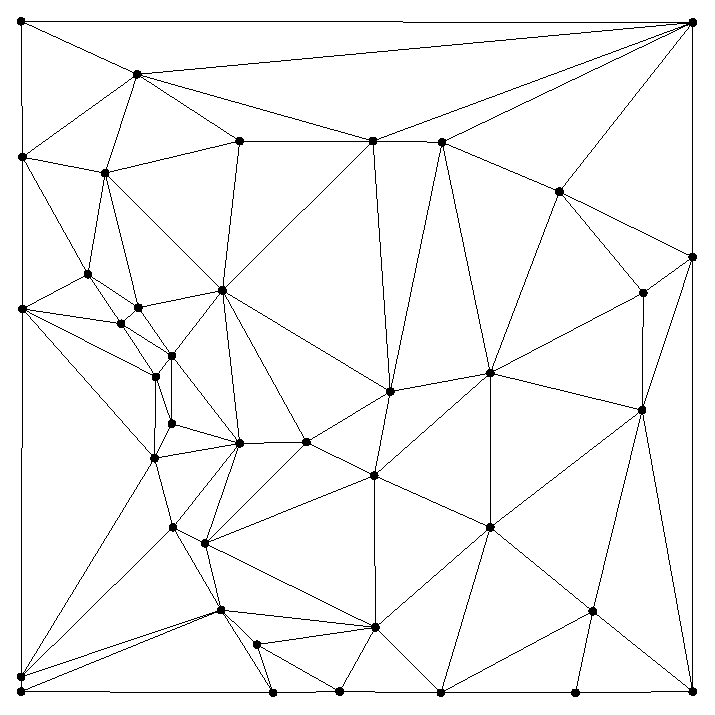
\includegraphics[width=0.4\textwidth]{delunolabel.eps}} \hspace{0.5cm} 
\subfigure[Triangulation after applying the label phase]{\label{fig:Labelphaseafter}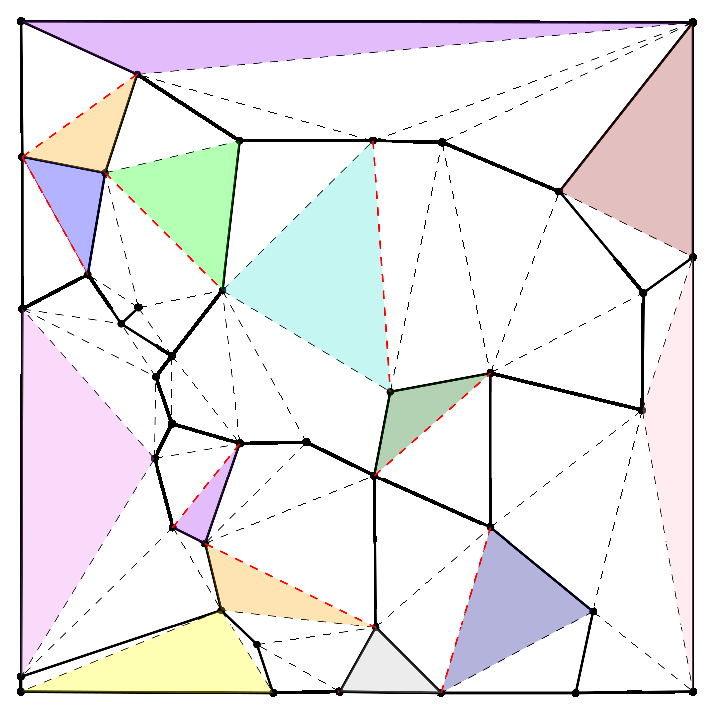
\includegraphics[width=0.4\textwidth]{labelandseedcolors.eps}}
\caption{Label phase: (a) Input Delaunay triangulation. (b) Solid lines are the frontier-edges, dashed lines are the internal-edges and colorful triangles are seed triangles. }
\label{figs:label_phase} 
\end{figure}

The final result of this step is shown in Figure \ref{figs:label_phase}. The colorful triangles will be used in the next phase as seed triangles to generate the polygons.  In Figure \ref{fig:Labelphaseafter} it can be also observed that terminal-edge regions are already formed and delimited by frontier-edges. 
%those edges are the edges of the final mesh.



%describir el etiquedado
%hacer un dibujo ql
%tula

\subsection{Travel Phase}
\label{subsec:Travelpohase}

In this phase polygons are recognized and represented as a closed polyline.  \textcolor{blue}{The main idea behind this phase is travel through adjacent triangles inside a terminal-edge region and save their frontier-edge as edges of the new polygon in counter clock wise order (ccw).}%to look for the frontier-edges of the triangles belonging to each terminal-edge region  in counter clock wise order (ccw). 

For this purpose, the algorithm  uses each triangle $t$ in the seed list created in the previous phase as the starting triangle to build each polygon. Note that every triangle can be used to generate a polygon, but we use one triangle adjacent to a terminal-edge to avoid generating the same polygon twice. 

\textcolor{blue}{Let be $t$ a triangle of the seed list and $P$ a temporary array to store a polygon, if $t$ has 3 frontier-edges, then $t$ is saved as a polygon in $P$, and the algorithm goes to the next triangle in the seed list, else, the algorithm stores the tree or two continuous endpoints of the edges of $t$ labeled as frontier-edge in $P$ in ccw, saves $t$ as a initial triangle, choose the first stored endpoint $v_{init}$ in $P$ as initial vertex (by lemma \ref{l:verticeslemma} each vertex of a terminal-edge region is part of a frontier-edge) and the last stored endpoint $v_{end}$ in $P$. After, the algorithm travels to the next adjacent triangle $t'$ in ccw that have $v_{end}$ as vertex. There are three cases for $t'$:}

%For this purpose, the algorithm  uses each triangle $t$ in the seed list created in the previous phase as the starting triangle to built each polygon. 
%The algorithm stores the frontier-edges of $t$ (if it has one), chooses one frontier-edge vertex as an initial point $v_{init}$ and the other as an endpoint $v_{end}$ and travel  through the next adjacent triangle $t'$ searching for new frontier edges. 
%The algorithm considers three following  cases for $t'$:


%decir como se inicia el viaje, con t triangulo inicial y t' el nuevo triangulo, con tres frontier edge es poligono.

%agregar el caso cuando por problemas de prescion no hay semilla



\begin{enumerate}[label=\roman*)]
    %comparte un arco con $t$, explicar con t' y t el anterior, t tiene un arco frontera y es endpoint de t', t' 
    \item \textcolor{blue}{ The triangle $t'$ has just 1 continuous frontier-edge $e$ that contains $v_{end}$. Then $e$ is store in $P$, $v_{end}$ is updated with last stored endpoint and the next triangle $t'$ is the next non-visited triangle that contains the new $v_{end}$.} % Then $t'$ shares an frontier-edge with the last triangle visited (where the last endpoint $v_{end}$ come from), and a frontier edge with a triangle that can be visited, the new $t'$ is that last no visited triangle.
    
    \item The triangle $t'$ is an ear triangle (a triangle with 2 frontier-edges). In this case, those both edges are stored in ccw in $P$, $v_{end}$ is updated with last stored endpoint and the last triangle visited is the new $t'$ because the other two triangles are adjacent by frontier-edges (i.e. They are in other terminal-edge region).
    
    \item The triangle $t'$ has no frontier edge. $t'$ shares an internal-edge with the last triangle visited and with other two triangles that can be visited, but just one of these contains the endpoint $v_{end}$ as vertex, so that triangle is the new $t'$. This case can occur when a barrier edge is found, when a triangle is between two ear triangles or when the algorithm surrounds an ear triangle of another terminal-edge region.
\end{enumerate}

The travel phase ends when $v_{end}$ reaches the initial point $v_{init}$ and the initial triangle $t$ is the same as $'t$. Experiments showed that both conditions are necessary, the first one due to a triangle can be visited multiple times in flat polygons and the second one due to barrier-edges can be omitted if only the first condition is used. An example of this phase is shown in Figure \ref{fig:travelphase}.

\begin{figure}[h]
    \centering
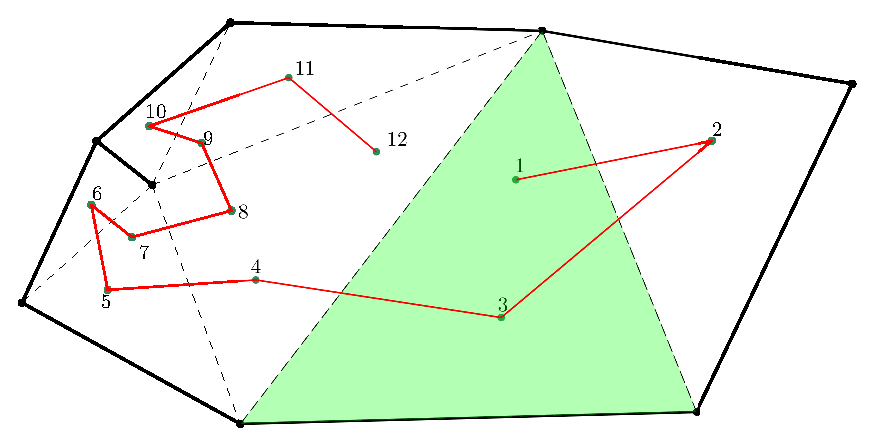
\includegraphics[width=0.5\textwidth]{travelphase2.eps}

    \caption{Travel of the algorithm inside a terminal-edge region. The green triangle is a seed triangle, the numbers indicate in which step of the iteration each triangle is visited. Note that triangles with no frontier-edge are visited 3 times, with 1 frontier-edge 2 times and with 2 frontier-edges 1 time.} 
    \label{fig:travelphase}
\end{figure}


After generating the polygon $P$, the algorithm checks if $P$ has barrier-edge tips. This can be easily done by just checking repetition of consecutive vertices in $P$. Given three consecutive vertices of $P$, $v_i$, $v_j$ and $v_k$. If $v_i$ and $v_k$ are equal, then $v_j$ is a barrier-edge tip. If $P$ does not have barrier-edge tips, then the polygon is saved as part of the mesh, else, the polygon is sent to the next of non-simple polygon reparation.



%Poner aquí imagen de los tres casos mñn uwu

\subsection{Non-simple polygon reparation}
\label{subsec:nonsimplereparation}

As we have mentioned, the generated polygons might be non-simple; this is the fact when they contain barrier-edges tips. In this section, we describe the algorithm to transform non-simple polygons into simple-ones by using the barrier-edges inside polygons and some additional internal-edges of the initial triangulation to build the new simple polygons. The use of any internal-edge allows us to split polygons as stated in Lemma \ref{l:verticeslemma}.

The process of reparation works similar to label phase and travel phase but inside a polygon $P$, \textcolor{blue}{ its exploits the lemma \ref{l:verticeslemma}, as all vertices inside the triangulation are part of a frontier-edge, then labeling as frontier-edge an internal-edge that contains a barrier-edge tip will generate two polytopes that can be used to generate two new polygons.} So the algorithm changes internal-edge to frontier-edges, saves seed triangles adjacent to those new frontier-edges, and uses them to generate new polygons, but instead of using a seed list, the algorithm generates a hash table $H$ with seeds triangle to generate polygons based on the original non-simple polygon $P$. 

The process is the following: For each barrier-edge tip $b_i$ in a polygon $P$, the algorithm count the number $deg(b_i)$ of incident internal-edges to $b_i$ in the original triangulation, if $deg(b_i)$ is odd then the algorithm labels the middle edge as frontier-edge, else, the algorithm chooses any of the middle edges to label as frontier-edge. In both cases, two triangles adjacent to the new frontier-edge are saved in a hash table $H$ to use one of them a seed triangle. \textcolor{blue}{Figure \ref{fig:betosplit} demonstrate an example of a polygon with three barrier-edge tips (vertices in green color). Figure \ref{fig:besplited} shows the as the middle internal-edge of all three barrier-edge tips is changed to a frontier-edge in order to generate the delimitation of the news polygons and six seeds triangles are saved in $H$.}


\begin{figure}[h]
\centering  
\resizebox{.8\linewidth}{!}{
   %%% not \center
\subfigure[] {\label{fig:betosplit}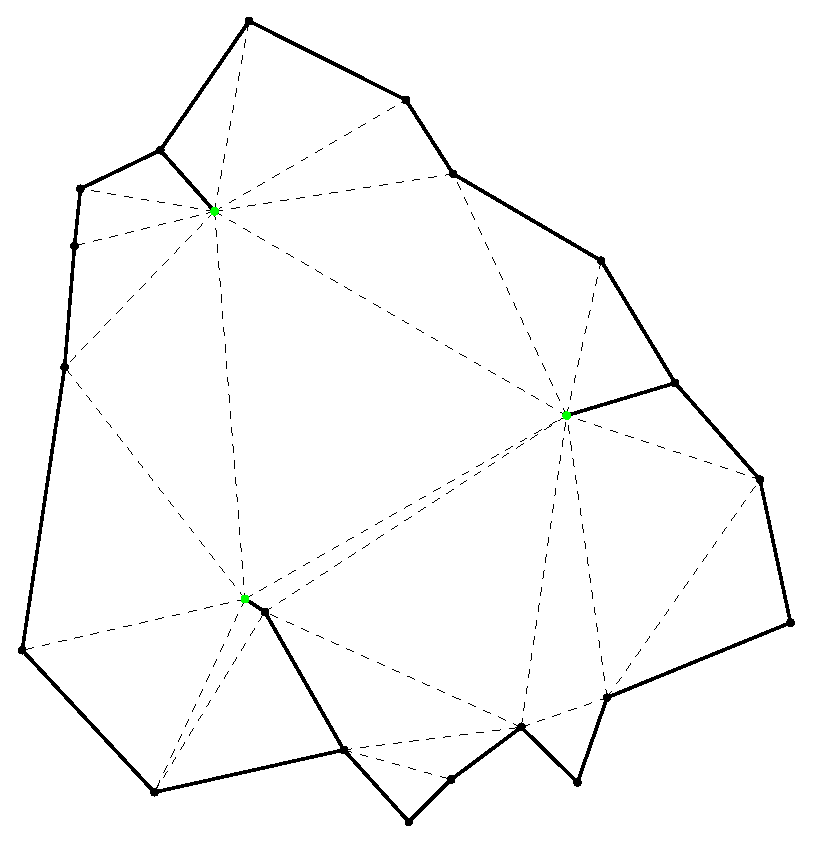
\includegraphics[width=0.3\textwidth, ]{be3split1.eps}}\hspace{0.5cm}
\subfigure[]{\label{fig:besplited}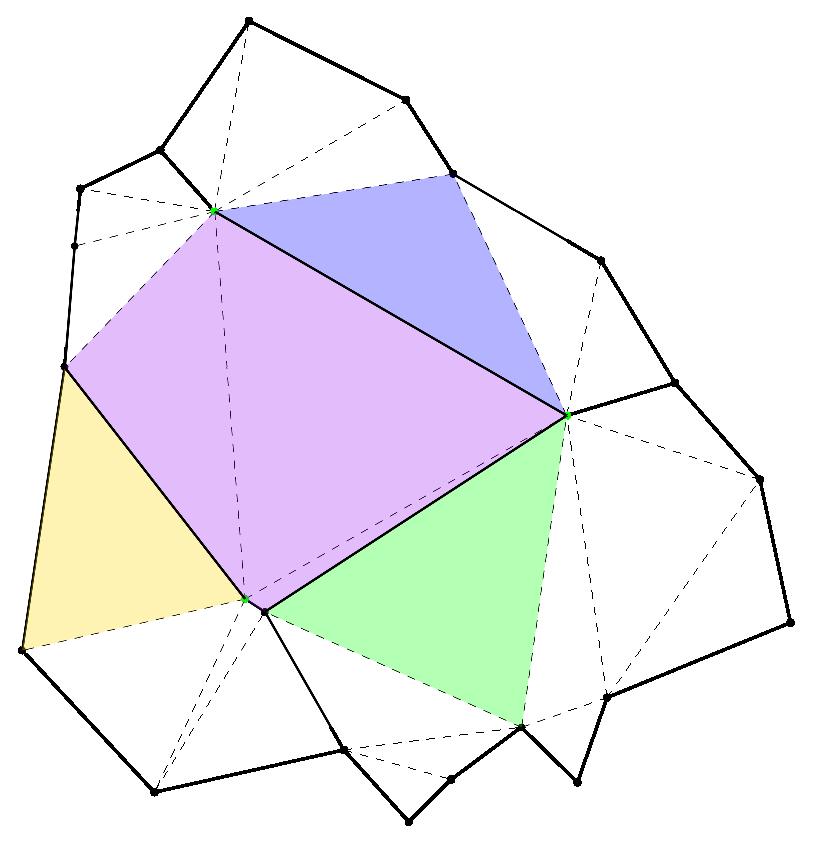
\includegraphics[width=0.3\textwidth]{be3split2v2.eps}}\hspace{0.5cm}
\subfigure[]{\label{fig:benewpolygons}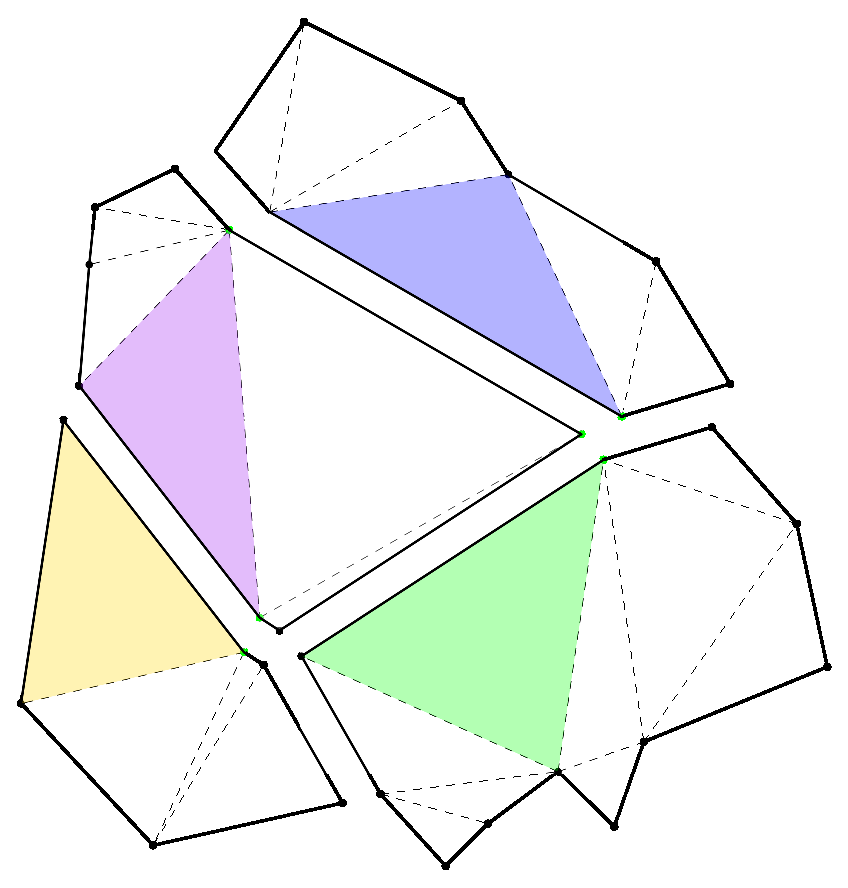
\includegraphics[width=0.3\textwidth]{be3split3v2.eps}}
}
\caption{Example of polygon split using barrier-edge tips. (a) Original polygon to split. (b) Middle edges incident to barrier-edge tips are label as frontier-edge and seed triangles (colorful triangles) are store in a hash table $H$ (c) Seeds triangles are used to generate new polygons without barrier-edge tips,  }
\label{figs:splitmid} 
\end{figure}

Later, the algorithm uses each triangle $t$ in the hash table $H$ to generate a new polygon, for each $t \in H$ the algorithm repeats the travel phase, but each triangle $t'$ reached during the travel is verified if $t'$ is in $H$. If it is the case, then the $'t$ is removed from $H$ to avoid generate the same polygon several times. \textcolor{blue}{This can be seen in Figure \ref{fig:besplited}, there are three purple triangles, but just one is chosen from $H$ to generate the new polygon, during its generation two purple triangles are removed from $H$ to avoid generate the same polygon again. Figure \ref{fig:besplited} shows the new polygon after the split and the seed triangles that generate them.}  %Figure \ref{fig:benewpolygons} shows the final result of use the travel phase with red triangles in  Figure \ref{fig:besplited}. 

The number of polygons generated after the split is at the most $(\#b + 1)$, with $\#b$ the number of barrier-edge tips in a polygon $P$. Figure \ref{figs:splitmid} explains the whole process.



% the algorithm takes care of selecting the best according to some quality criteria. 

%For each polygon $P$, the algorithm starts counting the number $\#b$ of barrier-edge tips. This is done by compare pair of continuous edges of the polygon and see if they are equal. If there isn't barrier-edge tips the polygon is saved as part of the mesh. Otherwise, the polygon is split to remove all the barrier-edges. 

%To repair non-simple polygons, the algorithm uses the barrier-edges and internal-edges of the triangulation to split them into simple ones. So, we avoid to check intersections between inserted edges and the polygon boundary.
%To split the polygon,  %the algorithm search by all the barrier-edge tips and label the middle edge of each one as a frontier-edge and save

%\textcolor{blue}{The algorithm uses the barrier-edges and internal-edges of the triangulation to split them into simple ones. So, we avoid to check intersections between inserted edges and the polygon boundary}. The process of splitting is the following: For each barrier-edge tip $b_i$ in a polygon $P$, the algorithm count the number $deg(b_i)$ of incident internal-edges to $b_i$ in the original triangulation, if $deg(b_i)$ is odd the algorithm label the middle edge as frontier-edge, else, the algorithm choose any of middle edges to label as frontier-edge. In both cases, two triangles adjacent to the edge are saved in a hash table $H$ to use one of them a seed.

%After, the algorithm uses the triangles in $H$ to generate new polygons without barrier-edge tips. For each triangle $t_i \in H$ is used the function showed in \S\ref{subsec:Travelpohase}, but for each new triangle $t'$ reached is verified if $t'$ is in $H$, in that case $t'$ is removed from $H$ to avoid use $t'$ as seed an repeat the same polygon.




%After, a iteration is made over all elements in the hash table $H$. 
% This process is shown in Figure \ref{figs:splitmid}.

%The process of split is the follow: For each barrier-edge tip $b_i$ in a polygon $P$, the algorithm count the number $deg(b_i)$ of adjacent internal-edges to $b_i$ in the original triangulation, if $deg(b_i)$ is odd the algorithm choose the middle edge to split the polygon, else, the algorithm choose any of middle edges to split the polygon. This process is shown in Figure \ref{figs:splitmid}.  



% - Se inicializa la tabla de hash
%- Se recorre todo el polytope buscando BET}
%- Cuando se encuentra uno, se busca la arista de almedio, se marca como un frontier-edge y se guardan sus dos triangulos adjyancetes en una tabla hash
% - Se usan los triangulos de la tabla de hash para generar los nuevos pligonos
% - Mientras se viaja a por el poligono, se verifica si este está en la tabla de hash, si lo está se elimina
% - Proceso se repite hasta que no hayan más triangulos en la tabla de hash.


%When a polygon $P$ is generated the algorithm count the number $\#b$ of barrier-edge tips, this is done by compare pair of continuous edges of the polygon and see if they are equal. If there isn't barrier-edge tips the polygon is saved as part of the mesh, else, the polygon is call to split in two recursively until remove all the barrier-edges. 

%The process of split is the follow: Be $b_i$ a barrier-edge tip in a polygon $P$, the algorithm count the number $deg(b_i)$ of adjacent edges to $b_i$ in the original triangulation, if $deg(b_i)$ is odd the algorithm choose the middle edge to split the polygon, else, the algorithm choose any of middle edges to split the polygon. This process is shown in Figure \ref{figs:splitmid}.



%The number of polygon generates after the split is at the most $(\#b + 1)$. The reason that this process is recursive is due to special cases where the edge choose to split $P$ contains two barrier-edge, so $#b$ needs to be calculate after each split.

\subsection{Computational Complexity Analysis}
\label{sub:Complexity Analysis}

In this section, we analyze the computational complexity of each phase and of the whole algorithm. Let  $n$ be the initial number of points, $m$ the number of triangles of the Delaunay triangulation, $k$ the number of triangles of the terminal-edge region used to generate the polygon $P$ and $\#b$ the number of barrier-edge tips of $P$.  

\begin{enumerate}
    \item[0.] \textbf{Initial Triangulation} The cost of generate a Delaunay Triangulation from a random set of points is $O(n\, log\, n)$.
    \item \textbf{Label Phase} This phase uses 3 iterations of cost $O(m)$, one to search max edges, other to label edges and another to save seed triangles.
    \item \textbf{Travel Phase} Build any polytope has cost $O(k)$, each triangle is visited at least 3 times in the worst case (when a triangle does not have a frontier-edge). As each terminal-edge region covers the whole domain without overlapping, then this phase has cost $O(m)$.
    % The complexity of this depends on the hash table and the polygon generation.
    \item \textbf{Non-simple polygon reparation phase} Check if a polygon has barrier-edge tips and calculates $deg(b_i)$ has cost $O(k)$ since the first one is an iteration over the number of vertices of the polygons and the second one the maximum number of triangles to count is $k$.  The max number of elements to save in the hash table is $2*\#b < k$, so building the hash table has a cost of $O(k)$, using an open hash, each search and deletion has a cost of $O(1)$. The cost of building the $O(\#b)$  new polygons cost $O(k)$, since new polygons uses the same $k$ numbers of triangles to be built, each triangle is just visited at least 3 times in the worst case. If all the polygons generated in travel phase have barrier-edge tips, this process has a final cost of $O(n)$.
%and the number of new polygons to generate is at least $(\#b + 1)$ .

\end{enumerate}

Finally the cost of the algorithm is $O(m)$, with $O(n\,log\,n)$ the cost of generating a initial triangulation.
    


%\subsection{Implementation Highlights}
%\label{subsec:highlights}
%Those are highlight to considerate in our implementations.

%\begin{enumerate}
   % \item To label edges as frontier-edge the algorithm mark the adjacency as $-1$. For example, in Figure \ref{figs:data_and_triangle}, to label red edge as frontier edge, $ADj_{3i+0}$ must change its value by $-1$. 

   % \item To improve the compute of $deg(b_i)$ we added an array that pair each vertex to one triangle adjacent to that vertex to the algorithm.

    %\item To the reparation phase a recursive function had been chosen to split polygons (split a polygon in two, and those two split them again until remove all barrier-edge tips), but to optimise the use of memory a open hash table was use. This table is an array of arbitrary length with pointers to linked list where save the seed triangles uses to generate the new polygons where each element is added to the begin of the linked list and each search operation has a delete operation inside to remove already use triangles.

%To the implementation of hash table, we use a open hash table 

%consist in two array, one contains the vertex of all polygons, and the second one and index array with the position of the last vertex of each polygon in the mesh.


%\end{enumerate}




\section{Terminal-edge regions based meshes vs Voronoi based meshes}
\label{sec:experimental_evaluation}

To show statistics about terminal-edge regions based meshes in contrast to a Voronoi diagram based mesh, we designed a simple experiment using a implementation of the algorithm in C++. 

\textcolor{blue}{The input of the experiment was generated with a initial point sets, those points are random points inserted inside a $2x2$ square. The number of points ranges from $10^1$ to $10^5$.} A tolerance $\pm \gamma$ is defined in case of a point $p$ is too close to one edge the square; in that case the point $p$ is inserted in the border edge instead. With those initial point sets were generates a set of Delaunay triangulation using Detri2 \cite{Detri2}. Results of the experiment are summarized in table \ref{table:results}. \textcolor{blue}{In the case of Voronoi meshes, Deldir \cite{deldir} was used to generate the geometric information of Clipped Voronoi diagram in Table \ref{table:resultsVoronoi}, using the same initial point sets as Voronoi sites.}

%After the point sets were generated, Detri2 \cite{Detri2} was used to build the Delaunay triangulation used as initial mesh to the implementation of the algorithm. Results of the experiment are summarized in table \ref{table:results}. Deldir \cite{deldir} was used to generate the geometric information of Clipped Voronoi diagram in Table \ref{table:resultsVoronoi}, using the same point sets as Voronoi sites.


\begin{table}
\centering
\resizebox{\columnwidth}{!}{%
\begin{tabular}{|r|r|r|r|r|r|r|r|}
\hline
\multicolumn{1}{|c|}{\begin{tabular}[c]{@{}c@{}}Input\\ points\end{tabular}} & \multicolumn{1}{c|}{\begin{tabular}[c]{@{}c@{}}Triangle\\ number\end{tabular}} & \multicolumn{1}{c|}{\begin{tabular}[c]{@{}c@{}}Terminal-edges\\ number\end{tabular}} & \multicolumn{1}{c|}{\begin{tabular}[c]{@{}c@{}}Terminal-edge\\ polygon\end{tabular}} & \multicolumn{1}{c|}{\begin{tabular}[c]{@{}c@{}}Max bet in \\ non-simple Polygons\end{tabular}} & \multicolumn{1}{c|}{Total Bet} & \multicolumn{1}{c|}{\begin{tabular}[c]{@{}c@{}}Triangles \\ per polygon\end{tabular}} & \multicolumn{1}{c|}{\begin{tabular}[c]{@{}c@{}}Edges \\ per polygon\end{tabular}} \\ \hline
10                                                                           & 14                                                                             & 5                                                                                    & 5                                                                                    & 0                                                                                              & 0                              & 2.80                                                                                  & 5.80                                                                              \\ \hline
$10^2$                                                                       & 192                                                                            & 34                                                                                   & 38                                                                                   & 2                                                                                              & 4                              & 5.05                                                                                  & 7.18                                                                              \\ \hline
$10^3$                                                                       & 1949                                                                           & 283                                                                                  & 310                                                                                  & 2                                                                                              & 27                             & 6.29                                                                                  & 8.30                                                                              \\ \hline
$10^4$                                                                       & 19618                                                                          & 3012                                                                                 & 3192                                                                                 & 4                                                                                              & 180                            & 6.15                                                                                  & 8.15                                                                              \\ \hline
$10^5$                                                                       & 197976                                                                         & 29965                                                                                & 31902                                                                                & 4                                                                                              & 1938                           & 6.21                                                                                  & 8.21                                                                              \\ \hline
\end{tabular}
}
\caption{Geometric information of polygon mesh }%\tiny{\footnotemark barrier-edge tips}}
\label{table:results}
\end{table}


\begin{table}
\centering
\begin{tabular}{|r|r|r|r|r|}
\hline
\multicolumn{1}{|c|}{\begin{tabular}[c]{@{}c@{}}Input \\ Points\end{tabular}} & \multicolumn{1}{c|}{\begin{tabular}[c]{@{}c@{}}Voronoi \\ vertices\end{tabular}} & \multicolumn{1}{c|}{\begin{tabular}[c]{@{}c@{}}Voronoit\\ Regions\end{tabular}} & \multicolumn{1}{c|}{\begin{tabular}[c]{@{}c@{}}Voronoi\\ Edges\end{tabular}} & \multicolumn{1}{c|}{\begin{tabular}[c]{@{}c@{}}Edges\\ per Region\end{tabular}} \\ \hline
10                                                                            & 22                                                                               & 10                                                                              & 31                                                                           & 4.9                                                                             \\ \hline
$10^2$                                                                        & 202                                                                              & 100                                                                             & 301                                                                          & 5.75                                                                            \\ \hline
$10^3$                                                                        & 2002                                                                             & 1000                                                                            & 3001                                                                         & 5.9                                                                             \\ \hline
$10^4$                                                                        & 20001                                                                            & 10000                                                                           & 30001                                                                        & 5.9618                                                                          \\ \hline
\end{tabular}
\caption{Geometric information of Clipped Voronoi diagram }%\tiny{\footnotemark barrier-edge tips}}
\label{table:resultsVoronoi}
\end{table}

%The input geometry can be  defined by the convex hull of  random point sets or  using a  PSLG specification. The Delaunay triangulations were generated using the  Detri2 library~\cite{Detri2}.  
%Table \ref{table:results} summarizes some   statistical data of the polygon meshes generated from random points.
In Table \label{table:results}, we can observe that after $10^4$ input points, the number of triangles per polygon is in average $6.5$ and the number of edges per polygon is $8.5$. The number of barrier-edges is less than $1\%$ of the number of points, so the reparation phase just adds $\approx 0.5\%$ of polygons to the mesh. If we compare these terminal-edge meshes with the meshes generated from the Voronoi diagram, the clipped Voronoi diagram contain 3 times more polygons than the our meshes. Each Voronoi region is formed by max 6 edges and, on average, terminal-edge polygons by 8 edges. 

Additionally, the terminal-edge regions meshes use only the points given as input; in contrast, the Voronoi based meshes use new points, the Voronoi points, one per each triangle of the Delaunay mesh. Since the number of triangles is greater than the number of input points, the size of the Voronoi mesh is greater than the size of the terminal-edge region mesh not only in terms of polygons but also in terms of mesh points.% COMO SE     VE ESTO EN LA TABLA?

The terminal-edge region based mesh does not need to insert extra-points to the boundary to fit the device geometry; in contrast the constrained  Voronoi based mesh needs to introduce new points at the boundary/interfaces to cut the Voronoi regions that go outside the domain.  


\begin{figure}[!h]
\centering     %%% not \center
\subfigure[Polygon Mesh]{\label{fig:polymesh}\includegraphics[width=0.3\textwidth]{1000points.png}} \hspace{0.5cm}
\subfigure[Voronoi diagram]{\label{fig:voromesh10000}\includegraphics[width=0.3\textwidth]{voronoicomparision.png}}
\caption{\textbf{(a)} Polygon mesh generated by 1000 random points.\textbf{(b)} Clipped Voronoi diagram of the same 1000 random points generated with Detri2QT \cite{Detri2}. }
\label{figs:voro_comp} 
\end{figure}


\begin{figure}[!h]
\centering     %%% not \center
\subfigure[Face PLSG from~\cite{Shewchuktriangle}]{\label{fig:PSLGface}\includegraphics[width=0.3\textwidth]{faceoriginalPSLG.png}} \hspace{0.5cm}
\subfigure[Face from Constrained Delaunay]{\label{fig:PSLGface26}\includegraphics[width=0.3\textwidth]{face26p.png}}\hspace{0.5cm}
\subfigure[Face from more refined triangulation]{\label{fig:PSLGface220}\includegraphics[width=0.3\textwidth]{facerefinement.png}}
\caption{\textcolor{blue}{\textbf{(a)} Original PLSG from~\cite{Shewchuktriangle} with 26 vertices, grey areas are holes. \textbf{(b)} Terminal-edge mesh version from a constrained Delaunay triangulation with the same 26 vertices. \textbf{(c)} Terminal-edge version of a refined Delaunay triangulation with 220 vertices.}}
\label{figs:facePSLG} 
\end{figure}


\begin{figure}[!h]
\centering     %%% not \center
\subfigure[Unicorn Triangulation]{\label{fig:PSLGUnicornTriangulation}\includegraphics[width=0.25\textwidth]{unicorntriangulation.png}}%
\subfigure[Unicorn Terminal-edge mesh]{\label{fig:PSLGUnicorn}\includegraphics[width=0.25\textwidth]{unicorn.png}}%
\subfigure[Clipped Voronoi unicorn]{\label{fig:PSLGUnicornVoronoi}\includegraphics[width=0.25\textwidth]{voronoiunicord.png}}%
\subfigure[Unicorn from more refined triangulation]{\label{fig:PSLGUnicorn100}\includegraphics[width=0.25\textwidth]{unicorn100.png}}

\caption{\textcolor{blue}{Comparision uniforn PLSG from \cite{AlejandroNUA2019} \textbf{(a)} Triangulation of unicorn PLSG with 36 vertices. \textbf{(b)} Terminal-edge mesh unicorn with 36 vertices. \textbf{(c)} Clipped Voronoi Unicorn PLSG with 100 vertices. \textbf{(d)} Terminal-edge mesh Unicorn from refined Delaunay triangulation with 100 vertices.}}
\label{figs:univornPSLG} 
\end{figure}

\textcolor{blue}{Figure~\ref{figs:voro_comp} is a comparison between terminal-edge mesh and Clipped Voronoi diagram. Both were generated with the same initial triangulation using DetriQT \cite{Detri2}. Figure~\ref{fig:polymesh} shows the polygon meshes generated by the proposed algorithm and Figure~\ref{fig:voromesh10000} a clipped Voronoi diagram. }

\textcolor{blue}{Figure \ref{figs:facePSLG} shows how more refinement triangulation as input affects to the output mesh. Figure \ref{fig:PSLGface} is a PLSG from~\cite{Shewchuktriangle} with 26 vertices. \ref{fig:PSLGface26} is a terminal-edge mesh generate using a constrained Delunay triangulation of \ref{fig:PSLGface26}. Figure \ref{fig:PSLGface220} uses a conforming Delaunay triangulation of  \ref{fig:PSLGface26} with a  maximum triangle area constraint of 100.}

\textcolor{blue}{Figure \ref{figs:univornPSLG} compares the terminal-edge mesh (Figure \ref{fig:PSLGUnicorn} and the clipped Voronoi mesh (Figure \ref{figs:univornPSLG}) of the same triangulation in Figure \ref{fig:PSLGUnicornTriangulation}. As Voronoi diagram mesh in Figure \ref{figs:univornPSLG} has in total 100  vertices, Figure \ref{fig:PSLGUnicorn100} shows the same unicorn generate from Delaunay refinement of Figure \ref{fig:PSLGUnicorn100} with of 100 vertices in total.}

%\textcolor{blue}{Figure~\ref{figs:PSLG} shows example of the terminal-edge mesh with PLSG as input and a comparison with clipped Voronoi mesh. Figure \ref{fig:PSLGface} is a classic PLSG from \cite{Shewchuktriangle} and Figures \ref{fig:PSLGUnicorn} and \ref{fig:PSLGUnicorn2} are PLSG from~\cite{AlejandroNUA2019}, both Figures have 36 vertices as input, but the Figure \ref{fig:PSLGUnicorn2} has in total 100 vertices as output. }

%Figure \ref{fig:PSLGface} is a PLSG obtained from~\cite{Shewchuktriangle} and Figures \ref{fig:AlejandroNUA2019} a is a PLSG obtained in from~\cite{ale}, both use the same number of vertices as the initial triangulation used by their generation, but Figure \ref{fig:PSLGface} added other 64 vertices to constrain the Voronoi cells inside the geometric domain.

%As an example of initial polygon meshes polygon meshes generated from PLSG geometries are shown in Figure . 





\section{Preliminary Simulation Results}
\label{sec:simulation_results}
In this section, we assess the terminal-edge region meshes in the virtual element method (VEM)~\cite{Basisprinciples}. To this end,
an L-shaped domain is considered. Fig.~\ref{figs:Lshaped} shows this domain meshed with a random and a semiuniform 
terminal-edge region sample mesh. The chosen problem is governed by the Laplace equation and
its exact solution is given by~\cite{MITCHELL2013350}
\begin{equation*}
u(x_1,x_2)=r^{2/3} \sin(2/3\,\theta), \quad r=\sqrt{x_1^2+x_2^2}, \quad \theta(x_1,x_2)=\arctan(x_2/x_1).
\end{equation*}
The boundary conditions are of Dirichlet type with the exact solution imposed on the entire domain boundary.
The re-entrant corner of the L-shaped domain introduces a singularity in the solution that manifests 
itself as unbounded derivatives of $u$ at the origin. The numerical solution (denoted by $u^h$) is assessed through
its convergence with mesh refinements. Figs.~\ref{figs:NormsLshapedRandom} and 
\ref{figs:NormsLshapedSemiuniform} present the $L^2$ norm and the $H^1$ seminorm
of the error, where it is shown that the optimal rates of convergence of 2 and 1 for the $L^2$ norm
and the $H^1$ seminorm of the error, respectively, are delivered by the VEM with random and 
semiuniform terminal-edge region meshes. Finally, contour plots of the VEM solution
for the $u$ field are shown in Fig.~\ref{figs:ContourPlots} for a random and a semiuniform mesh.

\begin{figure}[!bth]
\centering     %%% not \center
\subfigure[]{\label{fig:LshapedRandom}\includegraphics[width=0.48\textwidth]{Lshaped_random.png}} \hspace{0.1cm}
\subfigure[]{\label{fig:LshapedSemiuniform}\includegraphics[width=0.48\textwidth]{Lshaped_semiuniform.png}}
\caption{L-shaped domain meshed with \textbf{(a)} a random and \textbf{(b)} a semiuniform terminal-edge region mesh.}
\label{figs:Lshaped} 
\end{figure}

\begin{figure}[!bth]
\centering     %%% not \center
\subfigure[]{\label{fig:L2LshapedRandom}\includegraphics[width=0.4\textwidth]{L2_norm_random_Lshaped.png}} \hspace{0.5cm}
\subfigure[]{\label{fig:H1LshapedRandom}\includegraphics[width=0.4\textwidth]{H1_norm_random_Lshaped.png}}
\caption{\textbf{(a)} $L^2$ norm and \textbf{(b)} $H^1$ seminorm of the error for the L-shaped domain problem using the VEM and random terminal-edge region meshes.}
\label{figs:NormsLshapedRandom} 
\end{figure}

\begin{figure}[!bth]
\centering     %%% not \center
\subfigure[]{\label{fig:L2LshapedSemiuniform}\includegraphics[width=0.4\textwidth]{L2_norm_semiuniform_Lshaped.png}} \hspace{0.5cm}
\subfigure[]{\label{fig:H1LshapedSemiuniform}\includegraphics[width=0.4\textwidth]{H1_norm_semiuniform_Lshaped.png}}
\caption{\textbf{(a)} $L^2$ norm and \textbf{(b)} $H^1$ seminorm of the error for the L-shaped domain problem using the VEM and semiuniform terminal-edge region meshes.}
\label{figs:NormsLshapedSemiuniform} 
\end{figure}

\begin{figure}[!bth]
\centering     %%% not \center
\subfigure[]{\label{fig:ContourRandom}\includegraphics[width=0.45\textwidth]{contour_plot_random_Lshaped.png}} \hspace{0.5cm}
\subfigure[]{\label{fig:ContourSemiuniform}\includegraphics[width=0.45\textwidth]{contour_plot_semiuniform_Lshaped.png}}
\caption{Contour plots of the VEM solution for the $u$ field. \textbf{(a)} A random and \textbf{(b)} a semiuniform terminal-edge region mesh.}
\label{figs:ContourPlots} 
\end{figure}


% Authors must disclose all relationships or interests that 
% could have direct or potential influence or impart bias on 
% the work: 
%
% \section*{Conflict of interest}
%
% The authors declare that they have no conflict of interest.
\section{Conclusions and ongoing work}
\label{sec:conclusions}

We have presented a preliminary formalization and  statistical evaluation of a new kind of polygon mesh based on terminal-edge regions. We have observed that this kind of mesh contains three times less polygons and half the number of points than the standard polygon meshes based on the Voronoi diagram. 

We have shown some preliminary simulation results to show that this kind of mesh can be  as useful as Voronoi meshes with the VEM but using less  points and polygons. In 3D, where the number of tetrahedra in the worst case can be $O(n^2)$, with $n$ the number of input points, a stronger mesh point reduction should be obtained than in 2D. 

Until reciently, the mesh refinement had to be done in the input triangulation and the presented algorithm used to build the polygon mesh from that input. Since we keep the underline triangulation, we are planning to allow further refinement inside the polygon mesh in the next version of this polygon mesh generator. 

One of our hypothesis is that to take as input a Delaunay triangulation instead of any other triangulation should allow us to generate polygon meshes with less points and polygons. Thus,  our ongoing work is to complete the theoretical formulation and determine the scope these kind of mesh can be used. Since terminal edge-regions exist in 3D~\cite{HerviasHCF13}, we hope to soon have  a 3D polyhedron mesh generator.



% BibTeX users please use one of
%\bibliographystyle{spbasic}      % basic style, author-year citations


\bibliographystyle{spmpsci}      % mathematics and physical sciences
%\bibliographystyle{spfondecyt2021phys}       % APS-like style for physics
\bibliography{ref,polygonVem}   % name your BibTeX data base



\end{document}
% end of file template.tex

